%!TEX TS-program = xelatex
\documentclass[11pt]{article}

\usepackage[english]{babel}

\usepackage{amsmath,amssymb,amsfonts}
\usepackage[utf8]{inputenc}
\usepackage[T1]{fontenc}
\usepackage{stix2}
\usepackage[scaled]{helvet}
\usepackage[scaled]{inconsolata}

\usepackage{lastpage}

\usepackage{setspace}

\usepackage{ccicons}

\usepackage[hang,flushmargin]{footmisc}

\usepackage{geometry}

\setlength{\parindent}{0pt}
\setlength{\parskip}{6pt plus 2pt minus 1pt}

\usepackage{fancyhdr}
\renewcommand{\headrulewidth}{0pt}\providecommand{\tightlist}{%
  \setlength{\itemsep}{0pt}\setlength{\parskip}{0pt}}

\makeatletter
\newcounter{tableno}
\newenvironment{tablenos:no-prefix-table-caption}{
  \caption@ifcompatibility{}{
    \let\oldthetable\thetable
    \let\oldtheHtable\theHtable
    \renewcommand{\thetable}{tableno:\thetableno}
    \renewcommand{\theHtable}{tableno:\thetableno}
    \stepcounter{tableno}
    \captionsetup{labelformat=empty}
  }
}{
  \caption@ifcompatibility{}{
    \captionsetup{labelformat=default}
    \let\thetable\oldthetable
    \let\theHtable\oldtheHtable
    \addtocounter{table}{-1}
  }
}
\makeatother

\usepackage{array}
\newcommand{\PreserveBackslash}[1]{\let\temp=\\#1\let\\=\temp}
\let\PBS=\PreserveBackslash

\usepackage[breaklinks=true]{hyperref}
\hypersetup{colorlinks,%
citecolor=blue,%
filecolor=blue,%
linkcolor=blue,%
urlcolor=blue}
\usepackage{url}

\usepackage{caption}
\setcounter{secnumdepth}{0}
\usepackage{cleveref}

\usepackage{graphicx}
\makeatletter
\def\maxwidth{\ifdim\Gin@nat@width>\linewidth\linewidth
\else\Gin@nat@width\fi}
\makeatother
\let\Oldincludegraphics\includegraphics
\renewcommand{\includegraphics}[1]{\Oldincludegraphics[width=\maxwidth]{#1}}

\usepackage{longtable}
\usepackage{booktabs}

\usepackage{color}
\usepackage{fancyvrb}
\newcommand{\VerbBar}{|}
\newcommand{\VERB}{\Verb[commandchars=\\\{\}]}
\DefineVerbatimEnvironment{Highlighting}{Verbatim}{commandchars=\\\{\}}
% Add ',fontsize=\small' for more characters per line
\usepackage{framed}
\definecolor{shadecolor}{RGB}{248,248,248}
\newenvironment{Shaded}{\begin{snugshade}}{\end{snugshade}}
\newcommand{\KeywordTok}[1]{\textcolor[rgb]{0.13,0.29,0.53}{\textbf{#1}}}
\newcommand{\DataTypeTok}[1]{\textcolor[rgb]{0.13,0.29,0.53}{#1}}
\newcommand{\DecValTok}[1]{\textcolor[rgb]{0.00,0.00,0.81}{#1}}
\newcommand{\BaseNTok}[1]{\textcolor[rgb]{0.00,0.00,0.81}{#1}}
\newcommand{\FloatTok}[1]{\textcolor[rgb]{0.00,0.00,0.81}{#1}}
\newcommand{\ConstantTok}[1]{\textcolor[rgb]{0.00,0.00,0.00}{#1}}
\newcommand{\CharTok}[1]{\textcolor[rgb]{0.31,0.60,0.02}{#1}}
\newcommand{\SpecialCharTok}[1]{\textcolor[rgb]{0.00,0.00,0.00}{#1}}
\newcommand{\StringTok}[1]{\textcolor[rgb]{0.31,0.60,0.02}{#1}}
\newcommand{\VerbatimStringTok}[1]{\textcolor[rgb]{0.31,0.60,0.02}{#1}}
\newcommand{\SpecialStringTok}[1]{\textcolor[rgb]{0.31,0.60,0.02}{#1}}
\newcommand{\ImportTok}[1]{#1}
\newcommand{\CommentTok}[1]{\textcolor[rgb]{0.56,0.35,0.01}{\textit{#1}}}
\newcommand{\DocumentationTok}[1]{\textcolor[rgb]{0.56,0.35,0.01}{\textbf{\textit{#1}}}}
\newcommand{\AnnotationTok}[1]{\textcolor[rgb]{0.56,0.35,0.01}{\textbf{\textit{#1}}}}
\newcommand{\CommentVarTok}[1]{\textcolor[rgb]{0.56,0.35,0.01}{\textbf{\textit{#1}}}}
\newcommand{\OtherTok}[1]{\textcolor[rgb]{0.56,0.35,0.01}{#1}}
\newcommand{\FunctionTok}[1]{\textcolor[rgb]{0.00,0.00,0.00}{#1}}
\newcommand{\VariableTok}[1]{\textcolor[rgb]{0.00,0.00,0.00}{#1}}
\newcommand{\ControlFlowTok}[1]{\textcolor[rgb]{0.13,0.29,0.53}{\textbf{#1}}}
\newcommand{\OperatorTok}[1]{\textcolor[rgb]{0.81,0.36,0.00}{\textbf{#1}}}
\newcommand{\BuiltInTok}[1]{#1}
\newcommand{\ExtensionTok}[1]{#1}
\newcommand{\PreprocessorTok}[1]{\textcolor[rgb]{0.56,0.35,0.01}{\textit{#1}}}
\newcommand{\AttributeTok}[1]{\textcolor[rgb]{0.77,0.63,0.00}{#1}}
\newcommand{\RegionMarkerTok}[1]{#1}
\newcommand{\InformationTok}[1]{\textcolor[rgb]{0.56,0.35,0.01}{\textbf{\textit{#1}}}}
\newcommand{\WarningTok}[1]{\textcolor[rgb]{0.56,0.35,0.01}{\textbf{\textit{#1}}}}
\newcommand{\AlertTok}[1]{\textcolor[rgb]{0.94,0.16,0.16}{#1}}
\newcommand{\ErrorTok}[1]{\textcolor[rgb]{0.64,0.00,0.00}{\textbf{#1}}}
\newcommand{\NormalTok}[1]{#1}

\newlength{\cslhangindent}
\setlength{\cslhangindent}{1.5em}
\newlength{\csllabelwidth}
\setlength{\csllabelwidth}{3em}
\newenvironment{CSLReferences}[3] % #1 hanging-ident, #2 entry spacing
 {% don't indent paragraphs
  \setlength{\parindent}{0pt}
  % turn on hanging indent if param 1 is 1
  \ifodd #1 \everypar{\setlength{\hangindent}{\cslhangindent}}\ignorespaces\fi
  % set entry spacing
  \ifnum #2 > 0
  \setlength{\parskip}{#2\baselineskip}
  \fi
 }%
 {}
\usepackage{calc} % for \widthof, \maxof
\newcommand{\CSLBlock}[1]{#1\hfill\break}
\newcommand{\CSLLeftMargin}[1]{\parbox[t]{\maxof{\widthof{#1}}{\csllabelwidth}}{#1}}
\newcommand{\CSLRightInline}[1]{\parbox[t]{\linewidth}{#1}}
\newcommand{\CSLIndent}[1]{\hspace{\cslhangindent}#1}\geometry{verbose,letterpaper,tmargin=2.2cm,bmargin=2.2cm,lmargin=2.2cm,rmargin=2.2cm}

\usepackage{lineno}
\usepackage[nolists,noheads]{endfloat}

\pagestyle{plain}

\tolerance=1
\emergencystretch=\maxdimen
\hyphenpenalty=10000
\hbadness=10000

\doublespacing

\fancypagestyle{normal}
{
  \fancyhf{}
  \fancyfoot[R]{\footnotesize\sffamily\thepage\ of \pageref*{LastPage}}
}
\begin{document}
\raggedright
\thispagestyle{empty}
{\Large\bfseries\sffamily Thesis proposal}
\vskip 5em

%
\href{https://orcid.org/0000-0002-6506-6487}{Michael D.\,Catchen}%
%
\,\textsuperscript{1,2}

\textsuperscript{1}\,McGill University\quad \textsuperscript{2}\,Québec
Centre for Biodiversity Sciences


\textbf{Correspondance to:}\\
Michael D. Catchen --- \texttt{michael.catchen@mail.mcgill.ca}\\

\vfill
This work is released by its authors under a CC-BY 4.0 license\hfill\ccby\\
Last revision: \emph{\today}

\clearpage
\thispagestyle{empty}

\vfill
The proposal for my thesis, \emph{Simulation models for predictive
ecology}



\vfill

\clearpage
\linenumbers
\pagestyle{normal}

Within the last several hundred years, human activity has rapidly
reshaped both Earth's surface. These changes can roughly be divided into
two categories: (1) Land-use change, which has rapidly reshaped our
planet's surface and restructured habitats for every species, and (2)
climate change, words here, as a result of greenhouse gas emissions. As
a result \emph{ecological forecasting} (\textbf{dietze?}), or modeling
how ecological systems will change over time, has as an imperative to
mitigate the effect of these changes on Earth's ecosystems, their
functioning, and the services they provide to humans.

An oft applied definition of the origin of ecology is ``the application
of the scientific method to natural history.'' Since its origin ecology
has been a descriptive science. This is a natural biproduct of the
immense variability of Earth's biosphere.

In recent years, there has been an interest in an epistemological shift
in ecology. emerged to explain particular phenomena at particular
scales.

To shift ecology into a predictive science. The justification for this
shift is twofold: (1) bogged down philosophy of science, by further
rooting our understanding of ecosystem function and dynamics in an
ability to predict their structure (\textbf{PredictiveEcology?}). and
(2) the practical need for models for \emph{ecological forecasting}.

This term implicitly creates an analogy between predicting how
ecosystems will change in the future and weather forecasting. Use of
computational methods in NWP. Much as one would not aim to forecast the
weather to Quebec by applying Navier-Stokes. NWP has worked because it
incorporates information about data and meteorological processes
collected at difference scales into models that.

\begin{center}\rule{0.5\linewidth}{0.5pt}\end{center}

Historically the term ``theory,'' as applied in the physical sciences,
refers to mathematical models. Many (although not all) of these models
refers to a equation describing how the value of an observable state of
the system,
\(\begin{bmatrix}x_1 \\ x_2 \\ \vdots \end{bmatrix} = \vec{x}\), changes
as a function of time.

differential equations (in continuous time, difference equations for
discrete time)

Ecological processes vary across more variables than the tools of
analytic models are suited for. As the number of variables in an
analytic model increases, so does the ability of the scientist to decern
clear relationships between them. Chaotic dynamics emerge from simple
analytic models, and .

Whether ecosystems actually exhibit chaotic behavior is a different
question.

Until the 20th century, no theory of the gravitational dynamics of more
than 2 bodies. Understanding the gravitational dynamics of more than two
planets with any reliability proved difficult. Using the same models
(diffeqs), how could we adaquetly predict ecosystems?

\begin{center}\rule{0.5\linewidth}{0.5pt}\end{center}

Transition to theme of optimization given unknown information. A
forecast gives us a range of future values with uncertainty around them.
Further a convenient property that a forecasting model's uncertainty
goes up over time (if we assume the underlying process is Markov--this
is a strong assumption but oft true of the models we fit to temporal
data)

In face of uncertainty, decision making is an optimization problem. We
have some goal state for the future, and some estimate of what the state
of the world will be given a set of actions. Frame optimization problem
mathematically an introduce concept of solution-space and constraint.

Indeed Marx's most well known quote that ``philosophers have hitherto
only interpreted the world in various ways; the point is to change it.''

and a necessary step toward establishing a just and sustainable world.

Transition to specifics of this thesis.

\begin{figure}
\centering
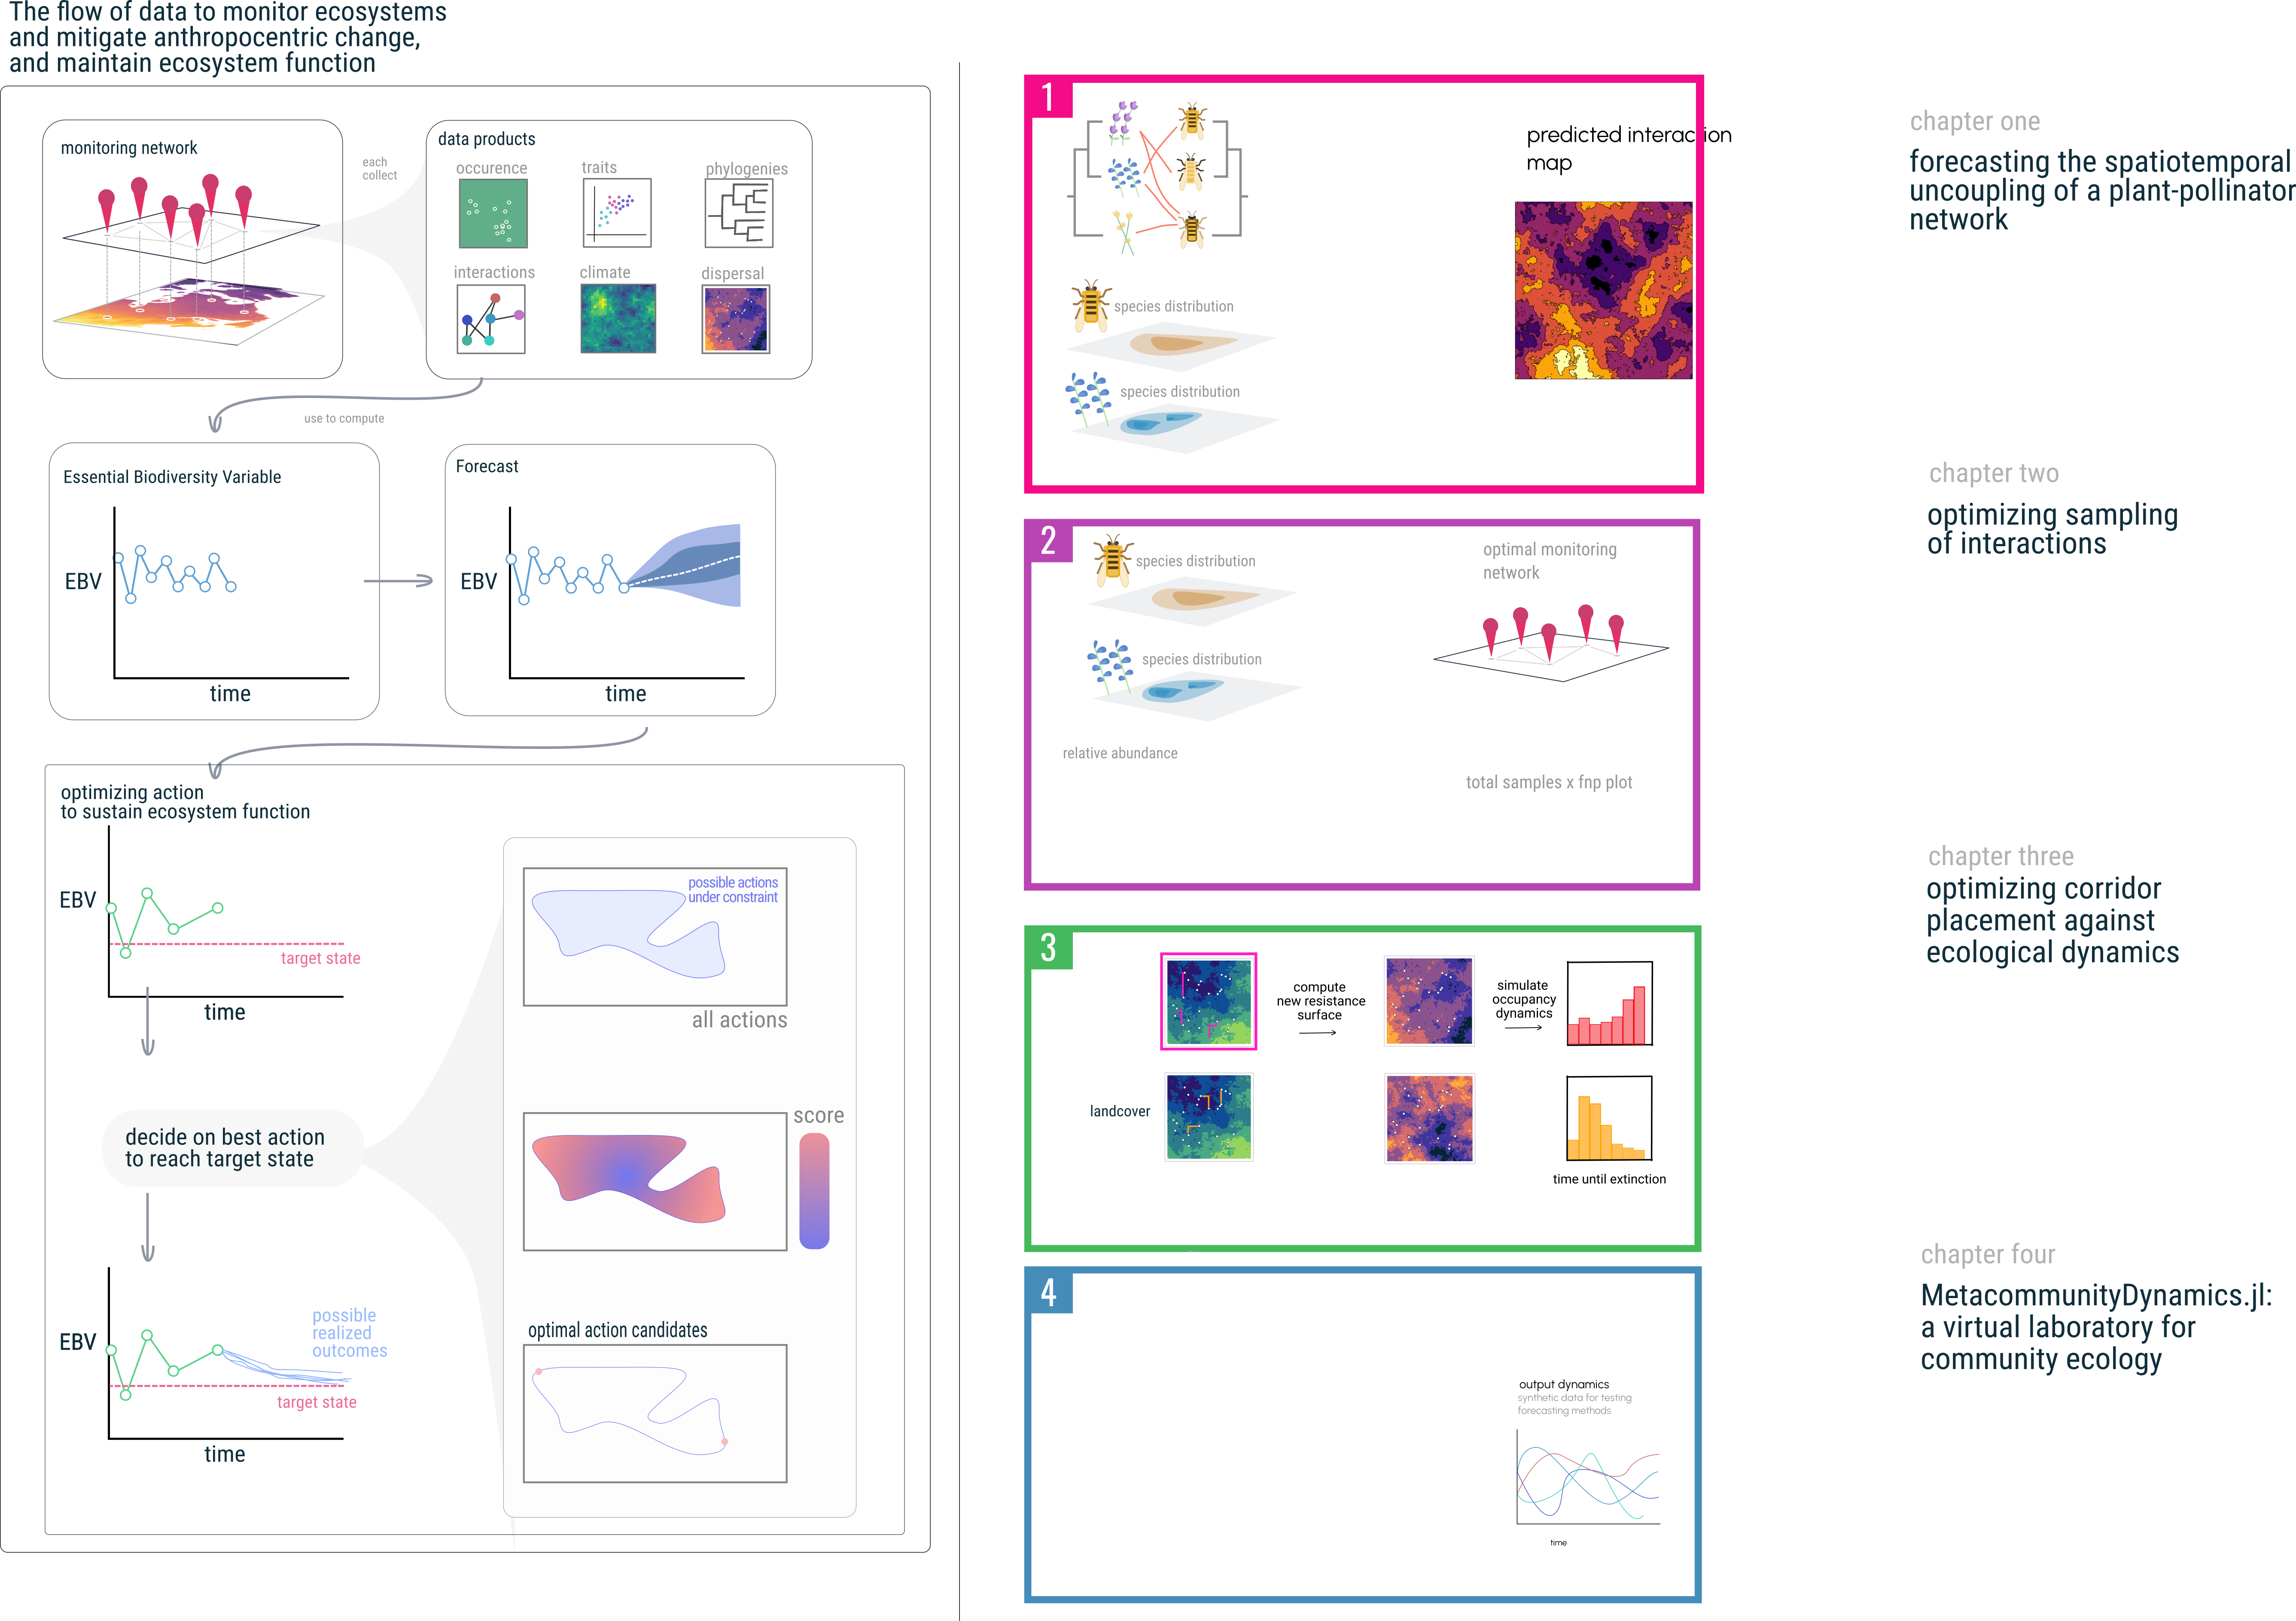
\includegraphics{./figures/thesisconcept.png}
\caption{thesis concept}
\end{figure}

\hypertarget{ch1-forecasting-the-phenological-uncoupling-of-a-plant-pollinator-network}{%
\section{CH1 Forecasting the phenological uncoupling of a
plant-pollinator
network}\label{ch1-forecasting-the-phenological-uncoupling-of-a-plant-pollinator-network}}

This chapter uses several years of data on bee-flower phenology and
interactions, combined with spatial records of species occurrence via
GBIF, to predict the probability of each realized interaction network as
a function of location and time.

\hypertarget{data}{%
\subsection{Data}\label{data}}

\hypertarget{methods}{%
\subsection{Methods}\label{methods}}

\begin{itemize}
\tightlist
\item
  simulate species distribution and efficacy of detection given a set of
  observation points where the dist from observation site decays.
\item
  optimize set of repeated sampling locations L for a \emph{known}
  distribution D.
\item
  address SDM not being the territory
\end{itemize}

\hypertarget{preliminary-results}{%
\subsection{Preliminary Results}\label{preliminary-results}}

Transition to next chapter by discussing uncertainty in interaction
prediction across space.

\hypertarget{ch2-optimizing-sampling-of-interactions}{%
\section{CH2 optimizing sampling of
interactions}\label{ch2-optimizing-sampling-of-interactions}}

This chapter discusses the effect of species relative abundance on
samples of interaction data, and proposes a method for optimizing
spatial sampling of a possible interaction between species as a function
of the estimated distribution of both species.

\hypertarget{methods-1}{%
\subsection{Methods}\label{methods-1}}

\begin{itemize}
\tightlist
\item
  the missing link paper, turn this into optimizing with two different
  SDMs
\end{itemize}

\hypertarget{results}{%
\subsection{Results}\label{results}}

\hypertarget{ch3-optimizing-corridor-placement}{%
\section{CH3 optimizing corridor
placement}\label{ch3-optimizing-corridor-placement}}

This chapter proposes an algorithm for optimizing
(corridorplacement/restoration effort) given a raster where each cell
indicates land-cover. The optimization method uses the result of a
simulated process (specifically occupancy dynamics in the landscape) and
uses simulated annealing to estimate the global optimum of the
targetstate (specfically mean-time-to-extinction for the occupancy
dynamics example).

\hypertarget{methods-2}{%
\section{Methods}\label{methods-2}}

\begin{itemize}
\tightlist
\item
  land cover -\textgreater{} resistance -\textgreater{} extinction time
\item
  simulated annealing to optimize landscape optimization
\end{itemize}

\hypertarget{ch4-a-software-note-on-the-resulting-packages.}{%
\section{CH4 a software note on the resulting
packages.}\label{ch4-a-software-note-on-the-resulting-packages.}}

(MetacommunityDynamics.jl: a virtual laboratory for community ecology):
a collection of modules in the Julia language for different aspects of
metacommunity ecology, including most of the code used for the preceding
chapters.

\begin{itemize}
\item
  TK conceptual figure with interfaces between what I'm writing / have
  contributed to and linked with other libraries
\item
  \texttt{Observatories.jl}, \texttt{Corridors.jl}, \texttt{MCD.jl}
\end{itemize}

\end{document}
